\documentclass[twoside]{book}

% Packages required by doxygen
\usepackage{fixltx2e}
\usepackage{calc}
\usepackage{doxygen}
\usepackage[export]{adjustbox} % also loads graphicx
\usepackage{graphicx}
\usepackage[utf8]{inputenc}
\usepackage{makeidx}
\usepackage{multicol}
\usepackage{multirow}
\PassOptionsToPackage{warn}{textcomp}
\usepackage{textcomp}
\usepackage[nointegrals]{wasysym}
\usepackage[table]{xcolor}

% Font selection
\usepackage[T1]{fontenc}
\usepackage[scaled=.90]{helvet}
\usepackage{courier}
\usepackage{amssymb}
\usepackage{sectsty}
\renewcommand{\familydefault}{\sfdefault}
\allsectionsfont{%
  \fontseries{bc}\selectfont%
  \color{darkgray}%
}
\renewcommand{\DoxyLabelFont}{%
  \fontseries{bc}\selectfont%
  \color{darkgray}%
}
\newcommand{\+}{\discretionary{\mbox{\scriptsize$\hookleftarrow$}}{}{}}

% Page & text layout
\usepackage{geometry}
\geometry{%
  a4paper,%
  top=2.5cm,%
  bottom=2.5cm,%
  left=2.5cm,%
  right=2.5cm%
}
\tolerance=750
\hfuzz=15pt
\hbadness=750
\setlength{\emergencystretch}{15pt}
\setlength{\parindent}{0cm}
\setlength{\parskip}{3ex plus 2ex minus 2ex}
\makeatletter
\renewcommand{\paragraph}{%
  \@startsection{paragraph}{4}{0ex}{-1.0ex}{1.0ex}{%
    \normalfont\normalsize\bfseries\SS@parafont%
  }%
}
\renewcommand{\subparagraph}{%
  \@startsection{subparagraph}{5}{0ex}{-1.0ex}{1.0ex}{%
    \normalfont\normalsize\bfseries\SS@subparafont%
  }%
}
\makeatother

% Headers & footers
\usepackage{fancyhdr}
\pagestyle{fancyplain}
\fancyhead[LE]{\fancyplain{}{\bfseries\thepage}}
\fancyhead[CE]{\fancyplain{}{}}
\fancyhead[RE]{\fancyplain{}{\bfseries\leftmark}}
\fancyhead[LO]{\fancyplain{}{\bfseries\rightmark}}
\fancyhead[CO]{\fancyplain{}{}}
\fancyhead[RO]{\fancyplain{}{\bfseries\thepage}}
\fancyfoot[LE]{\fancyplain{}{}}
\fancyfoot[CE]{\fancyplain{}{}}
\fancyfoot[RE]{\fancyplain{}{\bfseries\scriptsize Generated by Doxygen }}
\fancyfoot[LO]{\fancyplain{}{\bfseries\scriptsize Generated by Doxygen }}
\fancyfoot[CO]{\fancyplain{}{}}
\fancyfoot[RO]{\fancyplain{}{}}
\renewcommand{\footrulewidth}{0.4pt}
\renewcommand{\chaptermark}[1]{%
  \markboth{#1}{}%
}
\renewcommand{\sectionmark}[1]{%
  \markright{\thesection\ #1}%
}

% Indices & bibliography
\usepackage{natbib}
\usepackage[titles]{tocloft}
\setcounter{tocdepth}{3}
\setcounter{secnumdepth}{5}
\makeindex

% Hyperlinks (required, but should be loaded last)
\usepackage{ifpdf}
\ifpdf
  \usepackage[pdftex,pagebackref=true]{hyperref}
\else
  \usepackage[ps2pdf,pagebackref=true]{hyperref}
\fi
\hypersetup{%
  colorlinks=true,%
  linkcolor=blue,%
  citecolor=blue,%
  unicode%
}

% Custom commands
\newcommand{\clearemptydoublepage}{%
  \newpage{\pagestyle{empty}\cleardoublepage}%
}

\usepackage{caption}
\captionsetup{labelsep=space,justification=centering,font={bf},singlelinecheck=off,skip=4pt,position=top}

%===== C O N T E N T S =====

\begin{document}

% Titlepage & ToC
\hypersetup{pageanchor=false,
             bookmarksnumbered=true,
             pdfencoding=unicode
            }
\pagenumbering{alph}
\begin{titlepage}
\vspace*{7cm}
\begin{center}%
{\Large A\+E\+DA }\\
\vspace*{1cm}
{\large Generated by Doxygen 1.8.13}\\
\end{center}
\end{titlepage}
\clearemptydoublepage
\pagenumbering{roman}
\tableofcontents
\clearemptydoublepage
\pagenumbering{arabic}
\hypersetup{pageanchor=true}

%--- Begin generated contents ---
\chapter{R\+E\+A\+D\+ME}
\label{md___users_beamendes__documents__a_e_d_a__a_e_d_a-_f_e_u_p_aeda__r_e_a_d_m_e}
\Hypertarget{md___users_beamendes__documents__a_e_d_a__a_e_d_a-_f_e_u_p_aeda__r_e_a_d_m_e}
aeda 
\chapter{Hierarchical Index}
\section{Class Hierarchy}
This inheritance list is sorted roughly, but not completely, alphabetically\+:\begin{DoxyCompactList}
\item \contentsline{section}{Beach}{\pageref{class_beach}}{}
\begin{DoxyCompactList}
\item \contentsline{section}{Bayou\+Beach}{\pageref{class_bayou_beach}}{}
\item \contentsline{section}{River\+Beach}{\pageref{class_river_beach}}{}
\end{DoxyCompactList}
\item \contentsline{section}{Company}{\pageref{class_company}}{}
\item \contentsline{section}{Services}{\pageref{class_services}}{}
\end{DoxyCompactList}

\chapter{Class Index}
\section{Class List}
Here are the classes, structs, unions and interfaces with brief descriptions\+:\begin{DoxyCompactList}
\item\contentsline{section}{\hyperlink{class_bayou_beach}{Bayou\+Beach} }{\pageref{class_bayou_beach}}{}
\item\contentsline{section}{\hyperlink{class_beach}{Beach} }{\pageref{class_beach}}{}
\item\contentsline{section}{\hyperlink{class_company}{Company} }{\pageref{class_company}}{}
\item\contentsline{section}{\hyperlink{class_river_beach}{River\+Beach} }{\pageref{class_river_beach}}{}
\item\contentsline{section}{\hyperlink{class_services}{Services} }{\pageref{class_services}}{}
\end{DoxyCompactList}

\chapter{Class Documentation}
\hypertarget{class_bayou_beach}{}\section{Bayou\+Beach Class Reference}
\label{class_bayou_beach}\index{Bayou\+Beach@{Bayou\+Beach}}
Inheritance diagram for Bayou\+Beach\+:\begin{figure}[H]
\begin{center}
\leavevmode
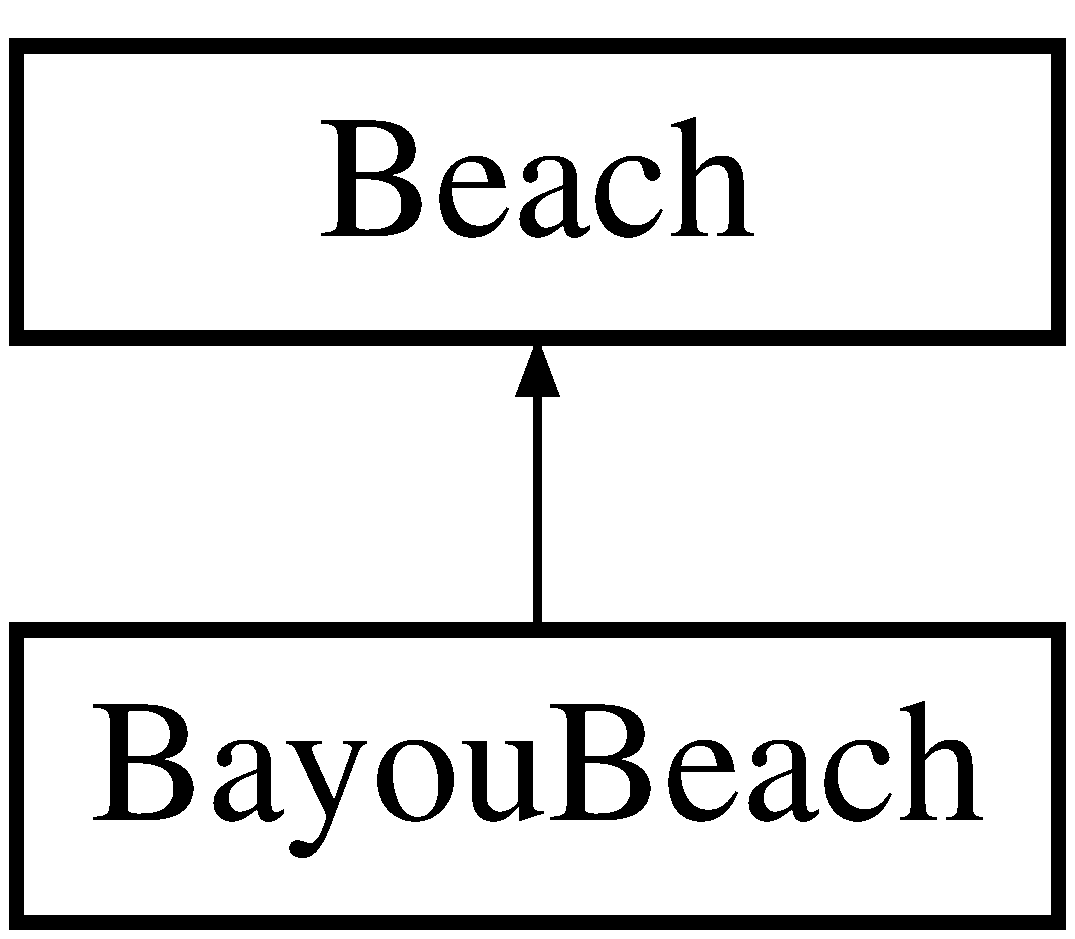
\includegraphics[height=2.000000cm]{class_bayou_beach}
\end{center}
\end{figure}
\subsection*{Public Member Functions}
\begin{DoxyCompactItemize}
\item 
\hyperlink{class_bayou_beach_a2d0c9a103748bbb90aaa772daa61f0c7}{Bayou\+Beach} (string \&county, string \&name, bool \&blueflag, bool \&lifeguard, unsigned long \&max\+\_\+capacity, float \&lat, float \&longi, float \&aquatic\+Area)
\begin{DoxyCompactList}\small\item\em Constructor class \hyperlink{class_bayou_beach}{Bayou\+Beach}. \end{DoxyCompactList}\item 
\hyperlink{class_bayou_beach_a8aa2c7bc67df6533807ef7e192ba8147}{Bayou\+Beach} (string beach)
\begin{DoxyCompactList}\small\item\em Helper construtor which recognizes and associates \hyperlink{class_beach}{Beach}\textquotesingle{}s object\textquotesingle{}s given attributes. \end{DoxyCompactList}\item 
string \hyperlink{class_bayou_beach_aad2b96c052075911ae3c0d23fd38b067}{get\+Type} () const
\begin{DoxyCompactList}\small\item\em Helps identifying from which derived class ths object is. \end{DoxyCompactList}\item 
float \hyperlink{class_bayou_beach_a4d4fe4911ac6772ac0335e133de498c8}{get\+\_\+width} () const
\item 
float \hyperlink{class_bayou_beach_a9187c703f1cb4e36831ca5e116ba758a}{get\+\_\+max\+Depth} () const
\item 
float \hyperlink{class_bayou_beach_ae2dc0496a300f7f8828a7b5898a68ee1}{get\+\_\+aquatic\+Area} () const
\item 
void \hyperlink{class_bayou_beach_a4bb316d56e931c219554b63a9ae68136}{set\+\_\+width} (float width)
\begin{DoxyCompactList}\small\item\em Changes width. \end{DoxyCompactList}\item 
void \hyperlink{class_bayou_beach_ada06dbcef6b191fc0413eca4bc5f7b65}{set\+\_\+max\+Depth} (float max\+Dept)
\begin{DoxyCompactList}\small\item\em Changes maximum depth. \end{DoxyCompactList}\item 
void \hyperlink{class_bayou_beach_a45c742927ddd735983e92a89c7baba96}{set\+\_\+aquatic\+Area} (float aquatic\+Area)
\begin{DoxyCompactList}\small\item\em Changes aquatic area. \end{DoxyCompactList}\item 
\mbox{\Hypertarget{class_bayou_beach_a4dc1d41b1884873288cb9e5fb567726f}\label{class_bayou_beach_a4dc1d41b1884873288cb9e5fb567726f}} 
void \hyperlink{class_bayou_beach_a4dc1d41b1884873288cb9e5fb567726f}{display\+Beach} ()
\begin{DoxyCompactList}\small\item\em Displays all information about the beach. \end{DoxyCompactList}\item 
void \hyperlink{class_bayou_beach_a16b3abbe3c2ebb1558d565f63178206a}{write\+Beach} (ofstream \&file) const
\begin{DoxyCompactList}\small\item\em Writes information about the beach in .txt file. \end{DoxyCompactList}\end{DoxyCompactItemize}
\subsection*{Additional Inherited Members}


\subsection{Constructor \& Destructor Documentation}
\mbox{\Hypertarget{class_bayou_beach_a2d0c9a103748bbb90aaa772daa61f0c7}\label{class_bayou_beach_a2d0c9a103748bbb90aaa772daa61f0c7}} 
\index{Bayou\+Beach@{Bayou\+Beach}!Bayou\+Beach@{Bayou\+Beach}}
\index{Bayou\+Beach@{Bayou\+Beach}!Bayou\+Beach@{Bayou\+Beach}}
\subsubsection{\texorpdfstring{Bayou\+Beach()}{BayouBeach()}\hspace{0.1cm}{\footnotesize\ttfamily [1/2]}}
{\footnotesize\ttfamily Bayou\+Beach\+::\+Bayou\+Beach (\begin{DoxyParamCaption}\item[{string \&}]{county,  }\item[{string \&}]{name,  }\item[{bool \&}]{blueflag,  }\item[{bool \&}]{lifeguard,  }\item[{unsigned long \&}]{max\+\_\+capacity,  }\item[{float \&}]{lat,  }\item[{float \&}]{longi,  }\item[{float \&}]{aquatic\+Area }\end{DoxyParamCaption})}



Constructor class \hyperlink{class_bayou_beach}{Bayou\+Beach}. 


\begin{DoxyParams}{Parameters}
{\em county} & \\
\hline
{\em name} & \\
\hline
{\em blueflag} & \\
\hline
{\em lifeguard} & \\
\hline
{\em max\+\_\+capacity} & \\
\hline
{\em lat} & \\
\hline
{\em longi} & \\
\hline
{\em aquatic\+Area} & \\
\hline
{\em basic\+Services} & \\
\hline
\end{DoxyParams}
\mbox{\Hypertarget{class_bayou_beach_a8aa2c7bc67df6533807ef7e192ba8147}\label{class_bayou_beach_a8aa2c7bc67df6533807ef7e192ba8147}} 
\index{Bayou\+Beach@{Bayou\+Beach}!Bayou\+Beach@{Bayou\+Beach}}
\index{Bayou\+Beach@{Bayou\+Beach}!Bayou\+Beach@{Bayou\+Beach}}
\subsubsection{\texorpdfstring{Bayou\+Beach()}{BayouBeach()}\hspace{0.1cm}{\footnotesize\ttfamily [2/2]}}
{\footnotesize\ttfamily Bayou\+Beach\+::\+Bayou\+Beach (\begin{DoxyParamCaption}\item[{string}]{beach }\end{DoxyParamCaption})}



Helper construtor which recognizes and associates \hyperlink{class_beach}{Beach}\textquotesingle{}s object\textquotesingle{}s given attributes. 


\begin{DoxyParams}{Parameters}
{\em line} & from txt file representing an object of class beach \\
\hline
\end{DoxyParams}


\subsection{Member Function Documentation}
\mbox{\Hypertarget{class_bayou_beach_ae2dc0496a300f7f8828a7b5898a68ee1}\label{class_bayou_beach_ae2dc0496a300f7f8828a7b5898a68ee1}} 
\index{Bayou\+Beach@{Bayou\+Beach}!get\+\_\+aquatic\+Area@{get\+\_\+aquatic\+Area}}
\index{get\+\_\+aquatic\+Area@{get\+\_\+aquatic\+Area}!Bayou\+Beach@{Bayou\+Beach}}
\subsubsection{\texorpdfstring{get\+\_\+aquatic\+Area()}{get\_aquaticArea()}}
{\footnotesize\ttfamily float Bayou\+Beach\+::get\+\_\+aquatic\+Area (\begin{DoxyParamCaption}{ }\end{DoxyParamCaption}) const\hspace{0.3cm}{\ttfamily [inline]}, {\ttfamily [virtual]}}

\begin{DoxyReturn}{Returns}
aquatic area 
\end{DoxyReturn}


Implements \hyperlink{class_beach_afc6a57f98777ec5de1882acaf2703e6d}{Beach}.

\mbox{\Hypertarget{class_bayou_beach_a9187c703f1cb4e36831ca5e116ba758a}\label{class_bayou_beach_a9187c703f1cb4e36831ca5e116ba758a}} 
\index{Bayou\+Beach@{Bayou\+Beach}!get\+\_\+max\+Depth@{get\+\_\+max\+Depth}}
\index{get\+\_\+max\+Depth@{get\+\_\+max\+Depth}!Bayou\+Beach@{Bayou\+Beach}}
\subsubsection{\texorpdfstring{get\+\_\+max\+Depth()}{get\_maxDepth()}}
{\footnotesize\ttfamily float Bayou\+Beach\+::get\+\_\+max\+Depth (\begin{DoxyParamCaption}{ }\end{DoxyParamCaption}) const\hspace{0.3cm}{\ttfamily [inline]}, {\ttfamily [virtual]}}

\begin{DoxyReturn}{Returns}
maximun depth 
\end{DoxyReturn}


Implements \hyperlink{class_beach_a5942f7aa56af3b61d2974a754913ab7e}{Beach}.

\mbox{\Hypertarget{class_bayou_beach_a4d4fe4911ac6772ac0335e133de498c8}\label{class_bayou_beach_a4d4fe4911ac6772ac0335e133de498c8}} 
\index{Bayou\+Beach@{Bayou\+Beach}!get\+\_\+width@{get\+\_\+width}}
\index{get\+\_\+width@{get\+\_\+width}!Bayou\+Beach@{Bayou\+Beach}}
\subsubsection{\texorpdfstring{get\+\_\+width()}{get\_width()}}
{\footnotesize\ttfamily float Bayou\+Beach\+::get\+\_\+width (\begin{DoxyParamCaption}{ }\end{DoxyParamCaption}) const\hspace{0.3cm}{\ttfamily [inline]}, {\ttfamily [virtual]}}

\begin{DoxyReturn}{Returns}
width; 
\end{DoxyReturn}


Implements \hyperlink{class_beach_af28e3603ea98766d94c9e8eb9f76d509}{Beach}.

\mbox{\Hypertarget{class_bayou_beach_aad2b96c052075911ae3c0d23fd38b067}\label{class_bayou_beach_aad2b96c052075911ae3c0d23fd38b067}} 
\index{Bayou\+Beach@{Bayou\+Beach}!get\+Type@{get\+Type}}
\index{get\+Type@{get\+Type}!Bayou\+Beach@{Bayou\+Beach}}
\subsubsection{\texorpdfstring{get\+Type()}{getType()}}
{\footnotesize\ttfamily string Bayou\+Beach\+::get\+Type (\begin{DoxyParamCaption}{ }\end{DoxyParamCaption}) const\hspace{0.3cm}{\ttfamily [inline]}, {\ttfamily [virtual]}}



Helps identifying from which derived class ths object is. 

\begin{DoxyReturn}{Returns}
\char`\"{}\+Bayou\+Beach\char`\"{} if it\textquotesingle{}s a class \hyperlink{class_bayou_beach}{Bayou\+Beach} object, \char`\"{}\+River\+Beach\char`\"{} if it\textquotesingle{}s a class \hyperlink{class_river_beach}{River\+Beach} object 
\end{DoxyReturn}


Implements \hyperlink{class_beach_a30001df535b2456e47611c7a0705660b}{Beach}.

\mbox{\Hypertarget{class_bayou_beach_a45c742927ddd735983e92a89c7baba96}\label{class_bayou_beach_a45c742927ddd735983e92a89c7baba96}} 
\index{Bayou\+Beach@{Bayou\+Beach}!set\+\_\+aquatic\+Area@{set\+\_\+aquatic\+Area}}
\index{set\+\_\+aquatic\+Area@{set\+\_\+aquatic\+Area}!Bayou\+Beach@{Bayou\+Beach}}
\subsubsection{\texorpdfstring{set\+\_\+aquatic\+Area()}{set\_aquaticArea()}}
{\footnotesize\ttfamily void Bayou\+Beach\+::set\+\_\+aquatic\+Area (\begin{DoxyParamCaption}\item[{float}]{aquatic\+Area }\end{DoxyParamCaption})\hspace{0.3cm}{\ttfamily [inline]}, {\ttfamily [virtual]}}



Changes aquatic area. 


\begin{DoxyParams}{Parameters}
{\em Aquatic} & area \\
\hline
\end{DoxyParams}


Implements \hyperlink{class_beach_a37e71c3348356d49f3b1080973708376}{Beach}.

\mbox{\Hypertarget{class_bayou_beach_ada06dbcef6b191fc0413eca4bc5f7b65}\label{class_bayou_beach_ada06dbcef6b191fc0413eca4bc5f7b65}} 
\index{Bayou\+Beach@{Bayou\+Beach}!set\+\_\+max\+Depth@{set\+\_\+max\+Depth}}
\index{set\+\_\+max\+Depth@{set\+\_\+max\+Depth}!Bayou\+Beach@{Bayou\+Beach}}
\subsubsection{\texorpdfstring{set\+\_\+max\+Depth()}{set\_maxDepth()}}
{\footnotesize\ttfamily void Bayou\+Beach\+::set\+\_\+max\+Depth (\begin{DoxyParamCaption}\item[{float}]{max\+Dept }\end{DoxyParamCaption})\hspace{0.3cm}{\ttfamily [inline]}, {\ttfamily [virtual]}}



Changes maximum depth. 


\begin{DoxyParams}{Parameters}
{\em maximum} & depth \\
\hline
\end{DoxyParams}


Implements \hyperlink{class_beach_af0226438bc6e731b2bca9f5a6078b572}{Beach}.

\mbox{\Hypertarget{class_bayou_beach_a4bb316d56e931c219554b63a9ae68136}\label{class_bayou_beach_a4bb316d56e931c219554b63a9ae68136}} 
\index{Bayou\+Beach@{Bayou\+Beach}!set\+\_\+width@{set\+\_\+width}}
\index{set\+\_\+width@{set\+\_\+width}!Bayou\+Beach@{Bayou\+Beach}}
\subsubsection{\texorpdfstring{set\+\_\+width()}{set\_width()}}
{\footnotesize\ttfamily void Bayou\+Beach\+::set\+\_\+width (\begin{DoxyParamCaption}\item[{float}]{width }\end{DoxyParamCaption})\hspace{0.3cm}{\ttfamily [inline]}, {\ttfamily [virtual]}}



Changes width. 


\begin{DoxyParams}{Parameters}
{\em width} & \\
\hline
\end{DoxyParams}


Implements \hyperlink{class_beach_a3f3a4bde9008bcc87861710e8c99c008}{Beach}.

\mbox{\Hypertarget{class_bayou_beach_a16b3abbe3c2ebb1558d565f63178206a}\label{class_bayou_beach_a16b3abbe3c2ebb1558d565f63178206a}} 
\index{Bayou\+Beach@{Bayou\+Beach}!write\+Beach@{write\+Beach}}
\index{write\+Beach@{write\+Beach}!Bayou\+Beach@{Bayou\+Beach}}
\subsubsection{\texorpdfstring{write\+Beach()}{writeBeach()}}
{\footnotesize\ttfamily void Bayou\+Beach\+::write\+Beach (\begin{DoxyParamCaption}\item[{ofstream \&}]{file }\end{DoxyParamCaption}) const\hspace{0.3cm}{\ttfamily [virtual]}}



Writes information about the beach in .txt file. 


\begin{DoxyParams}{Parameters}
{\em file} & \\
\hline
\end{DoxyParams}


Implements \hyperlink{class_beach_a2ba3bf80382fa1b5e00befe0c4ccde88}{Beach}.



The documentation for this class was generated from the following files\+:\begin{DoxyCompactItemize}
\item 
/\+Users/beamendes/\+Documents/\+A\+E\+D\+A/\+A\+E\+D\+A-\/\+F\+E\+U\+P/aeda/Beach.\+h\item 
/\+Users/beamendes/\+Documents/\+A\+E\+D\+A/\+A\+E\+D\+A-\/\+F\+E\+U\+P/aeda/Beach.\+cpp\end{DoxyCompactItemize}

\hypertarget{class_beach}{}\section{Beach Class Reference}
\label{class_beach}\index{Beach@{Beach}}
Inheritance diagram for Beach\+:\begin{figure}[H]
\begin{center}
\leavevmode
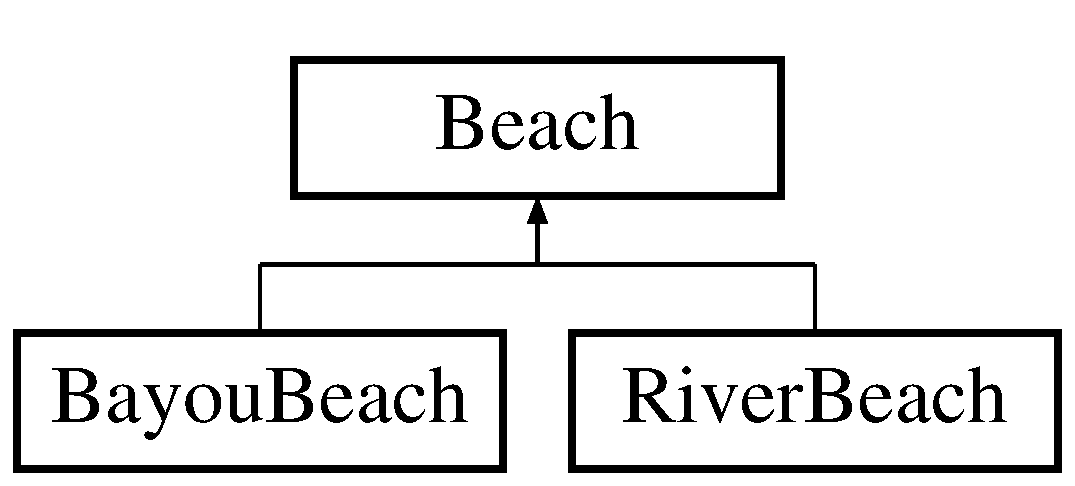
\includegraphics[height=2.000000cm]{class_beach}
\end{center}
\end{figure}
\subsection*{Public Member Functions}
\begin{DoxyCompactItemize}
\item 
\hyperlink{class_beach_addc648363a2a06c27983955cb1efe923}{Beach} (string \&county, string \&name, bool \&blueflag, bool \&lifeguard, unsigned long \&max\+\_\+capacity, float \&lat, float \&longi)
\begin{DoxyCompactList}\small\item\em Constructor for class \hyperlink{class_beach}{Beach}. \end{DoxyCompactList}\item 
\mbox{\Hypertarget{class_beach_a46f93d12e0399676c648d351613976af}\label{class_beach_a46f93d12e0399676c648d351613976af}} 
\hyperlink{class_beach_a46f93d12e0399676c648d351613976af}{Beach} ()
\begin{DoxyCompactList}\small\item\em Alternative constructor for class \hyperlink{class_beach}{Beach}. \end{DoxyCompactList}\item 
string \hyperlink{class_beach_ac25e8defc3ad46b44c64a908994bf43c}{get\+\_\+county} () const
\item 
string \hyperlink{class_beach_ae84e85693f8377673df6e91fba4503eb}{get\+\_\+name} () const
\item 
bool \hyperlink{class_beach_a6f3155d6b2a779d27b619d87775ff62b}{get\+\_\+blue\+\_\+flag} () const
\item 
bool \hyperlink{class_beach_a34d51732d2248a9000a8e7b09e377c5b}{get\+\_\+lifeguard} () const
\item 
unsigned long \hyperlink{class_beach_a428ee21d8889b86bd05f1460a0a1be34}{get\+\_\+max\+\_\+capacity} () const
\item 
float \hyperlink{class_beach_ae31a69a1f54505904331261db15ab3b6}{get\+\_\+latitude} () const
\item 
float \hyperlink{class_beach_a129633666198d102f58fe1dc7b9f89d8}{get\+\_\+longitude} () const
\item 
virtual float \hyperlink{class_beach_af28e3603ea98766d94c9e8eb9f76d509}{get\+\_\+width} () const =0
\item 
virtual float \hyperlink{class_beach_a5942f7aa56af3b61d2974a754913ab7e}{get\+\_\+max\+Depth} () const =0
\item 
virtual float \hyperlink{class_beach_afc6a57f98777ec5de1882acaf2703e6d}{get\+\_\+aquatic\+Area} () const =0
\item 
vector$<$ string $>$ \hyperlink{class_beach_a23305808d894c08a79fa3a0d201d0c51}{get\+Basic\+Services} () const
\item 
vector$<$ \hyperlink{class_services}{Services} $>$ \hyperlink{class_beach_a69ce8d1f21dc1b81edd6df001ec6c2b2}{get\+Extra\+Services} () const
\item 
virtual string \hyperlink{class_beach_a30001df535b2456e47611c7a0705660b}{get\+Type} () const =0
\begin{DoxyCompactList}\small\item\em Helps identifying from which derived class ths object is. \end{DoxyCompactList}\item 
void \hyperlink{class_beach_acfca41723a51e0da9596facfafe8f6db}{set\+\_\+name} (string name)
\begin{DoxyCompactList}\small\item\em Changes name. \end{DoxyCompactList}\item 
\mbox{\Hypertarget{class_beach_a019436b74c149f527a985f0c7c6fc8d2}\label{class_beach_a019436b74c149f527a985f0c7c6fc8d2}} 
void \hyperlink{class_beach_a019436b74c149f527a985f0c7c6fc8d2}{set\+\_\+blue\+\_\+flag} ()
\begin{DoxyCompactList}\small\item\em Changes blueflag. \end{DoxyCompactList}\item 
\mbox{\Hypertarget{class_beach_a861404c8f84396add0866190f1f83ecd}\label{class_beach_a861404c8f84396add0866190f1f83ecd}} 
void \hyperlink{class_beach_a861404c8f84396add0866190f1f83ecd}{set\+\_\+lifeguard} ()
\begin{DoxyCompactList}\small\item\em Changes lifeguard. \end{DoxyCompactList}\item 
void \hyperlink{class_beach_a952a4e75dd1e8200c6cc0bfde8728789}{set\+\_\+max\+\_\+capacity} (unsigned long max\+\_\+capacity)
\begin{DoxyCompactList}\small\item\em Changes maximum capacity. \end{DoxyCompactList}\item 
void \hyperlink{class_beach_a68a0fd1f91ee10e6acc9b676274bf2af}{set\+\_\+latitude} (float lat)
\begin{DoxyCompactList}\small\item\em Changes latitude. \end{DoxyCompactList}\item 
void \hyperlink{class_beach_af846ce1aabbd67742a4fef8fa64dcec8}{set\+\_\+longitude} (float longi)
\begin{DoxyCompactList}\small\item\em Changes longitude. \end{DoxyCompactList}\item 
void \hyperlink{class_beach_ae3e07bb07ec9c8b633ecb600c80567f2}{set\+\_\+\+Extra\+Services} (vector$<$ \hyperlink{class_services}{Services} $>$ \&extra\+Services)
\begin{DoxyCompactList}\small\item\em Changes extra services. \end{DoxyCompactList}\item 
virtual void \hyperlink{class_beach_a3f3a4bde9008bcc87861710e8c99c008}{set\+\_\+width} (float width)=0
\begin{DoxyCompactList}\small\item\em Changes width. \end{DoxyCompactList}\item 
virtual void \hyperlink{class_beach_af0226438bc6e731b2bca9f5a6078b572}{set\+\_\+max\+Depth} (float max\+Dept)=0
\begin{DoxyCompactList}\small\item\em Changes maximum depth. \end{DoxyCompactList}\item 
virtual void \hyperlink{class_beach_a37e71c3348356d49f3b1080973708376}{set\+\_\+aquatic\+Area} (float aquatic\+Area)=0
\begin{DoxyCompactList}\small\item\em Changes aquatic area. \end{DoxyCompactList}\item 
\mbox{\Hypertarget{class_beach_ae26aa5e34a3c7a85b297204f2d71fef3}\label{class_beach_ae26aa5e34a3c7a85b297204f2d71fef3}} 
double {\bfseries degrees\+To\+Radians} (double degrees)
\item 
double \hyperlink{class_beach_a4b7774165afd3ae88952281b9d846865}{distance\+To\+Beach} (float lat, float longi)
\begin{DoxyCompactList}\small\item\em Calculates distance from location\textquotesingle{}s G\+PS coordinates to beach\textquotesingle{}s coordinates. \end{DoxyCompactList}\item 
\mbox{\Hypertarget{class_beach_a05675f3e8c2523cc7db11aeb66933867}\label{class_beach_a05675f3e8c2523cc7db11aeb66933867}} 
virtual void \hyperlink{class_beach_a05675f3e8c2523cc7db11aeb66933867}{display\+Beach} ()=0
\begin{DoxyCompactList}\small\item\em Displays all information about the beach. \end{DoxyCompactList}\item 
void \hyperlink{class_beach_a242686b20a85f0efa8b19eafdb53d0a7}{add\+\_\+\+Basic\+Service} (string service)
\begin{DoxyCompactList}\small\item\em Adds Basic service to the vector. \end{DoxyCompactList}\item 
void \hyperlink{class_beach_a9182c63f32af1afd95649f14077c820c}{add\+\_\+\+Extra\+Service} (\hyperlink{class_services}{Services} service)
\begin{DoxyCompactList}\small\item\em Adds Extra service to the vector. \end{DoxyCompactList}\item 
void \hyperlink{class_beach_aa22b4abddf590bef4ff426f28866aca0}{erase\+\_\+\+Extra\+Service} (string service)
\begin{DoxyCompactList}\small\item\em Erase extra service from the vector. \end{DoxyCompactList}\item 
virtual void \hyperlink{class_beach_a2ba3bf80382fa1b5e00befe0c4ccde88}{write\+Beach} (ofstream \&file) const =0
\begin{DoxyCompactList}\small\item\em Writes information about the beach in .txt file. \end{DoxyCompactList}\end{DoxyCompactItemize}
\subsection*{Protected Attributes}
\begin{DoxyCompactItemize}
\item 
\mbox{\Hypertarget{class_beach_a5855b0e17ea41f7af6ed6633d0bb41cc}\label{class_beach_a5855b0e17ea41f7af6ed6633d0bb41cc}} 
string {\bfseries name}
\item 
\mbox{\Hypertarget{class_beach_a484973499734b3c2994385564adc2c81}\label{class_beach_a484973499734b3c2994385564adc2c81}} 
string {\bfseries county}
\item 
\mbox{\Hypertarget{class_beach_ac2d291e8784c9f0d8919134cf87ff5f0}\label{class_beach_ac2d291e8784c9f0d8919134cf87ff5f0}} 
bool {\bfseries blueflag}
\item 
\mbox{\Hypertarget{class_beach_a9625fc4212556b87b9e8389697ec9602}\label{class_beach_a9625fc4212556b87b9e8389697ec9602}} 
bool {\bfseries lifeguard}
\item 
\mbox{\Hypertarget{class_beach_a23bd6f845a6226cb173d6f505e480fc9}\label{class_beach_a23bd6f845a6226cb173d6f505e480fc9}} 
unsigned long {\bfseries max\+\_\+capacity}
\item 
\mbox{\Hypertarget{class_beach_ac3b74e09332b4605d20996434bdac781}\label{class_beach_ac3b74e09332b4605d20996434bdac781}} 
float {\bfseries lat}
\item 
\mbox{\Hypertarget{class_beach_a300efaac5c8a70309ad790378a61d809}\label{class_beach_a300efaac5c8a70309ad790378a61d809}} 
float {\bfseries longi}
\item 
\mbox{\Hypertarget{class_beach_a7b3208969cfa2492ac219cc7b8403717}\label{class_beach_a7b3208969cfa2492ac219cc7b8403717}} 
vector$<$ string $>$ {\bfseries basic\+Services}
\item 
\mbox{\Hypertarget{class_beach_a7f4fe9ab51968a44adf478b22b164364}\label{class_beach_a7f4fe9ab51968a44adf478b22b164364}} 
vector$<$ \hyperlink{class_services}{Services} $>$ {\bfseries extra\+Services}
\end{DoxyCompactItemize}


\subsection{Constructor \& Destructor Documentation}
\mbox{\Hypertarget{class_beach_addc648363a2a06c27983955cb1efe923}\label{class_beach_addc648363a2a06c27983955cb1efe923}} 
\index{Beach@{Beach}!Beach@{Beach}}
\index{Beach@{Beach}!Beach@{Beach}}
\subsubsection{\texorpdfstring{Beach()}{Beach()}}
{\footnotesize\ttfamily Beach\+::\+Beach (\begin{DoxyParamCaption}\item[{string \&}]{county,  }\item[{string \&}]{name,  }\item[{bool \&}]{blueflag,  }\item[{bool \&}]{lifeguard,  }\item[{unsigned long \&}]{max\+\_\+capacity,  }\item[{float \&}]{lat,  }\item[{float \&}]{longi }\end{DoxyParamCaption})}



Constructor for class \hyperlink{class_beach}{Beach}. 


\begin{DoxyParams}{Parameters}
{\em county} & \\
\hline
{\em name} & \\
\hline
{\em blueflag} & \\
\hline
{\em lifeguard} & \\
\hline
{\em max\+\_\+capacity} & \\
\hline
{\em lat} & \\
\hline
{\em longi} & \\
\hline
{\em basic\+Services} & \\
\hline
\end{DoxyParams}


\subsection{Member Function Documentation}
\mbox{\Hypertarget{class_beach_a242686b20a85f0efa8b19eafdb53d0a7}\label{class_beach_a242686b20a85f0efa8b19eafdb53d0a7}} 
\index{Beach@{Beach}!add\+\_\+\+Basic\+Service@{add\+\_\+\+Basic\+Service}}
\index{add\+\_\+\+Basic\+Service@{add\+\_\+\+Basic\+Service}!Beach@{Beach}}
\subsubsection{\texorpdfstring{add\+\_\+\+Basic\+Service()}{add\_BasicService()}}
{\footnotesize\ttfamily void Beach\+::add\+\_\+\+Basic\+Service (\begin{DoxyParamCaption}\item[{string}]{service }\end{DoxyParamCaption})}



Adds Basic service to the vector. 


\begin{DoxyParams}{Parameters}
{\em service} & \\
\hline
\end{DoxyParams}
\mbox{\Hypertarget{class_beach_a9182c63f32af1afd95649f14077c820c}\label{class_beach_a9182c63f32af1afd95649f14077c820c}} 
\index{Beach@{Beach}!add\+\_\+\+Extra\+Service@{add\+\_\+\+Extra\+Service}}
\index{add\+\_\+\+Extra\+Service@{add\+\_\+\+Extra\+Service}!Beach@{Beach}}
\subsubsection{\texorpdfstring{add\+\_\+\+Extra\+Service()}{add\_ExtraService()}}
{\footnotesize\ttfamily void Beach\+::add\+\_\+\+Extra\+Service (\begin{DoxyParamCaption}\item[{\hyperlink{class_services}{Services}}]{service }\end{DoxyParamCaption})}



Adds Extra service to the vector. 


\begin{DoxyParams}{Parameters}
{\em service} & \\
\hline
\end{DoxyParams}
\mbox{\Hypertarget{class_beach_a4b7774165afd3ae88952281b9d846865}\label{class_beach_a4b7774165afd3ae88952281b9d846865}} 
\index{Beach@{Beach}!distance\+To\+Beach@{distance\+To\+Beach}}
\index{distance\+To\+Beach@{distance\+To\+Beach}!Beach@{Beach}}
\subsubsection{\texorpdfstring{distance\+To\+Beach()}{distanceToBeach()}}
{\footnotesize\ttfamily double Beach\+::distance\+To\+Beach (\begin{DoxyParamCaption}\item[{float}]{lat,  }\item[{float}]{longi }\end{DoxyParamCaption})}



Calculates distance from location\textquotesingle{}s G\+PS coordinates to beach\textquotesingle{}s coordinates. 


\begin{DoxyParams}{Parameters}
{\em 2nd} & latitude \\
\hline
{\em 2nd} & longitude \\
\hline
\end{DoxyParams}
\begin{DoxyReturn}{Returns}
distance 
\end{DoxyReturn}
\mbox{\Hypertarget{class_beach_aa22b4abddf590bef4ff426f28866aca0}\label{class_beach_aa22b4abddf590bef4ff426f28866aca0}} 
\index{Beach@{Beach}!erase\+\_\+\+Extra\+Service@{erase\+\_\+\+Extra\+Service}}
\index{erase\+\_\+\+Extra\+Service@{erase\+\_\+\+Extra\+Service}!Beach@{Beach}}
\subsubsection{\texorpdfstring{erase\+\_\+\+Extra\+Service()}{erase\_ExtraService()}}
{\footnotesize\ttfamily void Beach\+::erase\+\_\+\+Extra\+Service (\begin{DoxyParamCaption}\item[{string}]{service }\end{DoxyParamCaption})}



Erase extra service from the vector. 


\begin{DoxyParams}{Parameters}
{\em service} & \\
\hline
\end{DoxyParams}
\mbox{\Hypertarget{class_beach_afc6a57f98777ec5de1882acaf2703e6d}\label{class_beach_afc6a57f98777ec5de1882acaf2703e6d}} 
\index{Beach@{Beach}!get\+\_\+aquatic\+Area@{get\+\_\+aquatic\+Area}}
\index{get\+\_\+aquatic\+Area@{get\+\_\+aquatic\+Area}!Beach@{Beach}}
\subsubsection{\texorpdfstring{get\+\_\+aquatic\+Area()}{get\_aquaticArea()}}
{\footnotesize\ttfamily virtual float Beach\+::get\+\_\+aquatic\+Area (\begin{DoxyParamCaption}{ }\end{DoxyParamCaption}) const\hspace{0.3cm}{\ttfamily [pure virtual]}}

\begin{DoxyReturn}{Returns}
aquatic area 
\end{DoxyReturn}


Implemented in \hyperlink{class_bayou_beach_ae2dc0496a300f7f8828a7b5898a68ee1}{Bayou\+Beach}, and \hyperlink{class_river_beach_a4bd144e5631968ed671051a203f1bce3}{River\+Beach}.

\mbox{\Hypertarget{class_beach_a6f3155d6b2a779d27b619d87775ff62b}\label{class_beach_a6f3155d6b2a779d27b619d87775ff62b}} 
\index{Beach@{Beach}!get\+\_\+blue\+\_\+flag@{get\+\_\+blue\+\_\+flag}}
\index{get\+\_\+blue\+\_\+flag@{get\+\_\+blue\+\_\+flag}!Beach@{Beach}}
\subsubsection{\texorpdfstring{get\+\_\+blue\+\_\+flag()}{get\_blue\_flag()}}
{\footnotesize\ttfamily bool Beach\+::get\+\_\+blue\+\_\+flag (\begin{DoxyParamCaption}{ }\end{DoxyParamCaption}) const}

\begin{DoxyReturn}{Returns}
1 if beach contains blue flag, 0 otherwise 
\end{DoxyReturn}
\mbox{\Hypertarget{class_beach_ac25e8defc3ad46b44c64a908994bf43c}\label{class_beach_ac25e8defc3ad46b44c64a908994bf43c}} 
\index{Beach@{Beach}!get\+\_\+county@{get\+\_\+county}}
\index{get\+\_\+county@{get\+\_\+county}!Beach@{Beach}}
\subsubsection{\texorpdfstring{get\+\_\+county()}{get\_county()}}
{\footnotesize\ttfamily string Beach\+::get\+\_\+county (\begin{DoxyParamCaption}{ }\end{DoxyParamCaption}) const}

\begin{DoxyReturn}{Returns}
county 
\end{DoxyReturn}
\mbox{\Hypertarget{class_beach_ae31a69a1f54505904331261db15ab3b6}\label{class_beach_ae31a69a1f54505904331261db15ab3b6}} 
\index{Beach@{Beach}!get\+\_\+latitude@{get\+\_\+latitude}}
\index{get\+\_\+latitude@{get\+\_\+latitude}!Beach@{Beach}}
\subsubsection{\texorpdfstring{get\+\_\+latitude()}{get\_latitude()}}
{\footnotesize\ttfamily float Beach\+::get\+\_\+latitude (\begin{DoxyParamCaption}{ }\end{DoxyParamCaption}) const}

\begin{DoxyReturn}{Returns}
latitude 
\end{DoxyReturn}
\mbox{\Hypertarget{class_beach_a34d51732d2248a9000a8e7b09e377c5b}\label{class_beach_a34d51732d2248a9000a8e7b09e377c5b}} 
\index{Beach@{Beach}!get\+\_\+lifeguard@{get\+\_\+lifeguard}}
\index{get\+\_\+lifeguard@{get\+\_\+lifeguard}!Beach@{Beach}}
\subsubsection{\texorpdfstring{get\+\_\+lifeguard()}{get\_lifeguard()}}
{\footnotesize\ttfamily bool Beach\+::get\+\_\+lifeguard (\begin{DoxyParamCaption}{ }\end{DoxyParamCaption}) const}

\begin{DoxyReturn}{Returns}
1 if beach contains lifeguard, 0 otherwise 
\end{DoxyReturn}
\mbox{\Hypertarget{class_beach_a129633666198d102f58fe1dc7b9f89d8}\label{class_beach_a129633666198d102f58fe1dc7b9f89d8}} 
\index{Beach@{Beach}!get\+\_\+longitude@{get\+\_\+longitude}}
\index{get\+\_\+longitude@{get\+\_\+longitude}!Beach@{Beach}}
\subsubsection{\texorpdfstring{get\+\_\+longitude()}{get\_longitude()}}
{\footnotesize\ttfamily float Beach\+::get\+\_\+longitude (\begin{DoxyParamCaption}{ }\end{DoxyParamCaption}) const}

\begin{DoxyReturn}{Returns}
longitude 
\end{DoxyReturn}
\mbox{\Hypertarget{class_beach_a428ee21d8889b86bd05f1460a0a1be34}\label{class_beach_a428ee21d8889b86bd05f1460a0a1be34}} 
\index{Beach@{Beach}!get\+\_\+max\+\_\+capacity@{get\+\_\+max\+\_\+capacity}}
\index{get\+\_\+max\+\_\+capacity@{get\+\_\+max\+\_\+capacity}!Beach@{Beach}}
\subsubsection{\texorpdfstring{get\+\_\+max\+\_\+capacity()}{get\_max\_capacity()}}
{\footnotesize\ttfamily unsigned long Beach\+::get\+\_\+max\+\_\+capacity (\begin{DoxyParamCaption}{ }\end{DoxyParamCaption}) const}

\begin{DoxyReturn}{Returns}
maximum capacity 
\end{DoxyReturn}
\mbox{\Hypertarget{class_beach_a5942f7aa56af3b61d2974a754913ab7e}\label{class_beach_a5942f7aa56af3b61d2974a754913ab7e}} 
\index{Beach@{Beach}!get\+\_\+max\+Depth@{get\+\_\+max\+Depth}}
\index{get\+\_\+max\+Depth@{get\+\_\+max\+Depth}!Beach@{Beach}}
\subsubsection{\texorpdfstring{get\+\_\+max\+Depth()}{get\_maxDepth()}}
{\footnotesize\ttfamily virtual float Beach\+::get\+\_\+max\+Depth (\begin{DoxyParamCaption}{ }\end{DoxyParamCaption}) const\hspace{0.3cm}{\ttfamily [pure virtual]}}

\begin{DoxyReturn}{Returns}
maximun depth 
\end{DoxyReturn}


Implemented in \hyperlink{class_bayou_beach_a9187c703f1cb4e36831ca5e116ba758a}{Bayou\+Beach}, and \hyperlink{class_river_beach_a0bb0a4f13ad1e2d7576d5ef641057e11}{River\+Beach}.

\mbox{\Hypertarget{class_beach_ae84e85693f8377673df6e91fba4503eb}\label{class_beach_ae84e85693f8377673df6e91fba4503eb}} 
\index{Beach@{Beach}!get\+\_\+name@{get\+\_\+name}}
\index{get\+\_\+name@{get\+\_\+name}!Beach@{Beach}}
\subsubsection{\texorpdfstring{get\+\_\+name()}{get\_name()}}
{\footnotesize\ttfamily string Beach\+::get\+\_\+name (\begin{DoxyParamCaption}{ }\end{DoxyParamCaption}) const}

\begin{DoxyReturn}{Returns}
name 
\end{DoxyReturn}
\mbox{\Hypertarget{class_beach_af28e3603ea98766d94c9e8eb9f76d509}\label{class_beach_af28e3603ea98766d94c9e8eb9f76d509}} 
\index{Beach@{Beach}!get\+\_\+width@{get\+\_\+width}}
\index{get\+\_\+width@{get\+\_\+width}!Beach@{Beach}}
\subsubsection{\texorpdfstring{get\+\_\+width()}{get\_width()}}
{\footnotesize\ttfamily virtual float Beach\+::get\+\_\+width (\begin{DoxyParamCaption}{ }\end{DoxyParamCaption}) const\hspace{0.3cm}{\ttfamily [pure virtual]}}

\begin{DoxyReturn}{Returns}
width; 
\end{DoxyReturn}


Implemented in \hyperlink{class_bayou_beach_a4d4fe4911ac6772ac0335e133de498c8}{Bayou\+Beach}, and \hyperlink{class_river_beach_a4fc528a34d80e3e2a6a48e53ab3e3f49}{River\+Beach}.

\mbox{\Hypertarget{class_beach_a23305808d894c08a79fa3a0d201d0c51}\label{class_beach_a23305808d894c08a79fa3a0d201d0c51}} 
\index{Beach@{Beach}!get\+Basic\+Services@{get\+Basic\+Services}}
\index{get\+Basic\+Services@{get\+Basic\+Services}!Beach@{Beach}}
\subsubsection{\texorpdfstring{get\+Basic\+Services()}{getBasicServices()}}
{\footnotesize\ttfamily vector$<$ string $>$ Beach\+::get\+Basic\+Services (\begin{DoxyParamCaption}{ }\end{DoxyParamCaption}) const}

\begin{DoxyReturn}{Returns}
vector of Basic beach services 
\end{DoxyReturn}
\mbox{\Hypertarget{class_beach_a69ce8d1f21dc1b81edd6df001ec6c2b2}\label{class_beach_a69ce8d1f21dc1b81edd6df001ec6c2b2}} 
\index{Beach@{Beach}!get\+Extra\+Services@{get\+Extra\+Services}}
\index{get\+Extra\+Services@{get\+Extra\+Services}!Beach@{Beach}}
\subsubsection{\texorpdfstring{get\+Extra\+Services()}{getExtraServices()}}
{\footnotesize\ttfamily vector$<$ \hyperlink{class_services}{Services} $>$ Beach\+::get\+Extra\+Services (\begin{DoxyParamCaption}{ }\end{DoxyParamCaption}) const}

\begin{DoxyReturn}{Returns}
vector of Extra beach services 
\end{DoxyReturn}
\mbox{\Hypertarget{class_beach_a30001df535b2456e47611c7a0705660b}\label{class_beach_a30001df535b2456e47611c7a0705660b}} 
\index{Beach@{Beach}!get\+Type@{get\+Type}}
\index{get\+Type@{get\+Type}!Beach@{Beach}}
\subsubsection{\texorpdfstring{get\+Type()}{getType()}}
{\footnotesize\ttfamily virtual string Beach\+::get\+Type (\begin{DoxyParamCaption}{ }\end{DoxyParamCaption}) const\hspace{0.3cm}{\ttfamily [pure virtual]}}



Helps identifying from which derived class ths object is. 

\begin{DoxyReturn}{Returns}
\char`\"{}\+Bayou\+Beach\char`\"{} if it\textquotesingle{}s a class \hyperlink{class_bayou_beach}{Bayou\+Beach} object, \char`\"{}\+River\+Beach\char`\"{} if it\textquotesingle{}s a class \hyperlink{class_river_beach}{River\+Beach} object 
\end{DoxyReturn}


Implemented in \hyperlink{class_bayou_beach_aad2b96c052075911ae3c0d23fd38b067}{Bayou\+Beach}, and \hyperlink{class_river_beach_a07f48c077de96aca001f47ce06253f2f}{River\+Beach}.

\mbox{\Hypertarget{class_beach_a37e71c3348356d49f3b1080973708376}\label{class_beach_a37e71c3348356d49f3b1080973708376}} 
\index{Beach@{Beach}!set\+\_\+aquatic\+Area@{set\+\_\+aquatic\+Area}}
\index{set\+\_\+aquatic\+Area@{set\+\_\+aquatic\+Area}!Beach@{Beach}}
\subsubsection{\texorpdfstring{set\+\_\+aquatic\+Area()}{set\_aquaticArea()}}
{\footnotesize\ttfamily virtual void Beach\+::set\+\_\+aquatic\+Area (\begin{DoxyParamCaption}\item[{float}]{aquatic\+Area }\end{DoxyParamCaption})\hspace{0.3cm}{\ttfamily [pure virtual]}}



Changes aquatic area. 


\begin{DoxyParams}{Parameters}
{\em Aquatic} & area \\
\hline
\end{DoxyParams}


Implemented in \hyperlink{class_bayou_beach_a45c742927ddd735983e92a89c7baba96}{Bayou\+Beach}, and \hyperlink{class_river_beach_ac236cb64cc422eea722bb99fdb29d4d0}{River\+Beach}.

\mbox{\Hypertarget{class_beach_ae3e07bb07ec9c8b633ecb600c80567f2}\label{class_beach_ae3e07bb07ec9c8b633ecb600c80567f2}} 
\index{Beach@{Beach}!set\+\_\+\+Extra\+Services@{set\+\_\+\+Extra\+Services}}
\index{set\+\_\+\+Extra\+Services@{set\+\_\+\+Extra\+Services}!Beach@{Beach}}
\subsubsection{\texorpdfstring{set\+\_\+\+Extra\+Services()}{set\_ExtraServices()}}
{\footnotesize\ttfamily void Beach\+::set\+\_\+\+Extra\+Services (\begin{DoxyParamCaption}\item[{vector$<$ \hyperlink{class_services}{Services} $>$ \&}]{extra\+Services }\end{DoxyParamCaption})}



Changes extra services. 


\begin{DoxyParams}{Parameters}
{\em extra\+Services} & \\
\hline
\end{DoxyParams}
\mbox{\Hypertarget{class_beach_a68a0fd1f91ee10e6acc9b676274bf2af}\label{class_beach_a68a0fd1f91ee10e6acc9b676274bf2af}} 
\index{Beach@{Beach}!set\+\_\+latitude@{set\+\_\+latitude}}
\index{set\+\_\+latitude@{set\+\_\+latitude}!Beach@{Beach}}
\subsubsection{\texorpdfstring{set\+\_\+latitude()}{set\_latitude()}}
{\footnotesize\ttfamily void Beach\+::set\+\_\+latitude (\begin{DoxyParamCaption}\item[{float}]{lat }\end{DoxyParamCaption})}



Changes latitude. 


\begin{DoxyParams}{Parameters}
{\em latitude} & \\
\hline
\end{DoxyParams}
\mbox{\Hypertarget{class_beach_af846ce1aabbd67742a4fef8fa64dcec8}\label{class_beach_af846ce1aabbd67742a4fef8fa64dcec8}} 
\index{Beach@{Beach}!set\+\_\+longitude@{set\+\_\+longitude}}
\index{set\+\_\+longitude@{set\+\_\+longitude}!Beach@{Beach}}
\subsubsection{\texorpdfstring{set\+\_\+longitude()}{set\_longitude()}}
{\footnotesize\ttfamily void Beach\+::set\+\_\+longitude (\begin{DoxyParamCaption}\item[{float}]{longi }\end{DoxyParamCaption})}



Changes longitude. 


\begin{DoxyParams}{Parameters}
{\em longitude} & \\
\hline
\end{DoxyParams}
\mbox{\Hypertarget{class_beach_a952a4e75dd1e8200c6cc0bfde8728789}\label{class_beach_a952a4e75dd1e8200c6cc0bfde8728789}} 
\index{Beach@{Beach}!set\+\_\+max\+\_\+capacity@{set\+\_\+max\+\_\+capacity}}
\index{set\+\_\+max\+\_\+capacity@{set\+\_\+max\+\_\+capacity}!Beach@{Beach}}
\subsubsection{\texorpdfstring{set\+\_\+max\+\_\+capacity()}{set\_max\_capacity()}}
{\footnotesize\ttfamily void Beach\+::set\+\_\+max\+\_\+capacity (\begin{DoxyParamCaption}\item[{unsigned long}]{max\+\_\+capacity }\end{DoxyParamCaption})}



Changes maximum capacity. 


\begin{DoxyParams}{Parameters}
{\em maximum} & capacity \\
\hline
\end{DoxyParams}
\mbox{\Hypertarget{class_beach_af0226438bc6e731b2bca9f5a6078b572}\label{class_beach_af0226438bc6e731b2bca9f5a6078b572}} 
\index{Beach@{Beach}!set\+\_\+max\+Depth@{set\+\_\+max\+Depth}}
\index{set\+\_\+max\+Depth@{set\+\_\+max\+Depth}!Beach@{Beach}}
\subsubsection{\texorpdfstring{set\+\_\+max\+Depth()}{set\_maxDepth()}}
{\footnotesize\ttfamily virtual void Beach\+::set\+\_\+max\+Depth (\begin{DoxyParamCaption}\item[{float}]{max\+Dept }\end{DoxyParamCaption})\hspace{0.3cm}{\ttfamily [pure virtual]}}



Changes maximum depth. 


\begin{DoxyParams}{Parameters}
{\em maximum} & depth \\
\hline
\end{DoxyParams}


Implemented in \hyperlink{class_bayou_beach_ada06dbcef6b191fc0413eca4bc5f7b65}{Bayou\+Beach}, and \hyperlink{class_river_beach_a1118c334abeeae8352ecaf0f33059f6a}{River\+Beach}.

\mbox{\Hypertarget{class_beach_acfca41723a51e0da9596facfafe8f6db}\label{class_beach_acfca41723a51e0da9596facfafe8f6db}} 
\index{Beach@{Beach}!set\+\_\+name@{set\+\_\+name}}
\index{set\+\_\+name@{set\+\_\+name}!Beach@{Beach}}
\subsubsection{\texorpdfstring{set\+\_\+name()}{set\_name()}}
{\footnotesize\ttfamily void Beach\+::set\+\_\+name (\begin{DoxyParamCaption}\item[{string}]{name }\end{DoxyParamCaption})}



Changes name. 


\begin{DoxyParams}{Parameters}
{\em name} & \\
\hline
\end{DoxyParams}
\mbox{\Hypertarget{class_beach_a3f3a4bde9008bcc87861710e8c99c008}\label{class_beach_a3f3a4bde9008bcc87861710e8c99c008}} 
\index{Beach@{Beach}!set\+\_\+width@{set\+\_\+width}}
\index{set\+\_\+width@{set\+\_\+width}!Beach@{Beach}}
\subsubsection{\texorpdfstring{set\+\_\+width()}{set\_width()}}
{\footnotesize\ttfamily virtual void Beach\+::set\+\_\+width (\begin{DoxyParamCaption}\item[{float}]{width }\end{DoxyParamCaption})\hspace{0.3cm}{\ttfamily [pure virtual]}}



Changes width. 


\begin{DoxyParams}{Parameters}
{\em width} & \\
\hline
\end{DoxyParams}


Implemented in \hyperlink{class_bayou_beach_a4bb316d56e931c219554b63a9ae68136}{Bayou\+Beach}, and \hyperlink{class_river_beach_a53697d96e65d8841e5979d3f5d79c9e3}{River\+Beach}.

\mbox{\Hypertarget{class_beach_a2ba3bf80382fa1b5e00befe0c4ccde88}\label{class_beach_a2ba3bf80382fa1b5e00befe0c4ccde88}} 
\index{Beach@{Beach}!write\+Beach@{write\+Beach}}
\index{write\+Beach@{write\+Beach}!Beach@{Beach}}
\subsubsection{\texorpdfstring{write\+Beach()}{writeBeach()}}
{\footnotesize\ttfamily virtual void Beach\+::write\+Beach (\begin{DoxyParamCaption}\item[{ofstream \&}]{file }\end{DoxyParamCaption}) const\hspace{0.3cm}{\ttfamily [pure virtual]}}



Writes information about the beach in .txt file. 


\begin{DoxyParams}{Parameters}
{\em file} & \\
\hline
\end{DoxyParams}


Implemented in \hyperlink{class_bayou_beach_a16b3abbe3c2ebb1558d565f63178206a}{Bayou\+Beach}, and \hyperlink{class_river_beach_acdbf29ab6540a2b0a5fd18cbea14375b}{River\+Beach}.



The documentation for this class was generated from the following files\+:\begin{DoxyCompactItemize}
\item 
/\+Users/beamendes/\+Documents/\+A\+E\+D\+A/\+A\+E\+D\+A-\/\+F\+E\+U\+P/aeda/Beach.\+h\item 
/\+Users/beamendes/\+Documents/\+A\+E\+D\+A/\+A\+E\+D\+A-\/\+F\+E\+U\+P/aeda/Beach.\+cpp\end{DoxyCompactItemize}

\hypertarget{class_company}{}\section{Company Class Reference}
\label{class_company}\index{Company@{Company}}
\subsection*{Public Member Functions}
\begin{DoxyCompactItemize}
\item 
\hyperlink{class_company_a29937dda711b09df306ae7ca9b3d6b42}{Company} ()
\item 
vector$<$ \hyperlink{class_beach}{Beach} $\ast$ $>$ \hyperlink{class_company_a5551b69f0b6de3037f7a3a4ca4d3c48a}{get\+Beaches} ()
\item 
\mbox{\Hypertarget{class_company_a637bea6b73fee60679b2786c7be03694}\label{class_company_a637bea6b73fee60679b2786c7be03694}} 
void \hyperlink{class_company_a637bea6b73fee60679b2786c7be03694}{add\+Beach} ()
\begin{DoxyCompactList}\small\item\em Adds beach to Beaches\textquotesingle{} vector with user\textquotesingle{}s input information. \end{DoxyCompactList}\item 
\mbox{\Hypertarget{class_company_a3936079f764ee1b095389eb526511e85}\label{class_company_a3936079f764ee1b095389eb526511e85}} 
void \hyperlink{class_company_a3936079f764ee1b095389eb526511e85}{remove\+Beach} ()
\begin{DoxyCompactList}\small\item\em Removes beach to Beaches\textquotesingle{} vector with user\textquotesingle{}s input information. \end{DoxyCompactList}\item 
void \hyperlink{class_company_a584718d76eabe565779c41f3d047eb77}{alter\+R\+Beach\+Info} (unsigned int option, unsigned int i)
\begin{DoxyCompactList}\small\item\em Alters river beach to Beaches\textquotesingle{} vector with user\textquotesingle{}s input information. \end{DoxyCompactList}\item 
void \hyperlink{class_company_a77499b6ff8a4913bdb00843613467e56}{alter\+B\+Beach\+Info} (unsigned int option, unsigned int i)
\begin{DoxyCompactList}\small\item\em Alters bayou beach to Beaches\textquotesingle{} vector with user\textquotesingle{}s input information. \end{DoxyCompactList}\item 
\mbox{\Hypertarget{class_company_ade7da5185959ac2ec280f94381a4c531}\label{class_company_ade7da5185959ac2ec280f94381a4c531}} 
void \hyperlink{class_company_ade7da5185959ac2ec280f94381a4c531}{add\+Service} ()
\begin{DoxyCompactList}\small\item\em Adds a service to a certain beach. \end{DoxyCompactList}\item 
\mbox{\Hypertarget{class_company_a0ec21ed7be545ec7154e0c2295ce804c}\label{class_company_a0ec21ed7be545ec7154e0c2295ce804c}} 
void \hyperlink{class_company_a0ec21ed7be545ec7154e0c2295ce804c}{alter\+Service} ()
\begin{DoxyCompactList}\small\item\em Alters a service. \end{DoxyCompactList}\item 
\mbox{\Hypertarget{class_company_a1c64f4273adb50b24e1cb2bf2c05ac08}\label{class_company_a1c64f4273adb50b24e1cb2bf2c05ac08}} 
void \hyperlink{class_company_a1c64f4273adb50b24e1cb2bf2c05ac08}{erase\+Service} ()
\begin{DoxyCompactList}\small\item\em Erases a service from a certain beach. \end{DoxyCompactList}\item 
int \hyperlink{class_company_afabcb7d6b8e6fdb49ce4c9352ac88287}{beach\+Exists} (string name)
\begin{DoxyCompactList}\small\item\em Verifies if beach with certain name exist. \end{DoxyCompactList}\item 
\mbox{\Hypertarget{class_company_ad740b440f2fa9948324c0aa0fa6d026e}\label{class_company_ad740b440f2fa9948324c0aa0fa6d026e}} 
void \hyperlink{class_company_ad740b440f2fa9948324c0aa0fa6d026e}{display\+Beaches} ()
\begin{DoxyCompactList}\small\item\em Displays the information about all beaches. \end{DoxyCompactList}\item 
\mbox{\Hypertarget{class_company_ad8d5d9aba5b078ca69fbc3f40b2bd282}\label{class_company_ad8d5d9aba5b078ca69fbc3f40b2bd282}} 
void \hyperlink{class_company_ad8d5d9aba5b078ca69fbc3f40b2bd282}{update\+File} ()
\begin{DoxyCompactList}\small\item\em Updates the file containing the information about the beaches according to the changes made in the program. \end{DoxyCompactList}\item 
\mbox{\Hypertarget{class_company_a9b7797f2e7b3bc31d1d2c6b7c79d703e}\label{class_company_a9b7797f2e7b3bc31d1d2c6b7c79d703e}} 
void \hyperlink{class_company_a9b7797f2e7b3bc31d1d2c6b7c79d703e}{search\+County} ()
\begin{DoxyCompactList}\small\item\em Searchs beach by county and displays its information. \end{DoxyCompactList}\item 
\mbox{\Hypertarget{class_company_a914fcef89a30b4a28cc4455183dab791}\label{class_company_a914fcef89a30b4a28cc4455183dab791}} 
void \hyperlink{class_company_a914fcef89a30b4a28cc4455183dab791}{search\+Name} ()
\begin{DoxyCompactList}\small\item\em Search beach by name and displays its information. \end{DoxyCompactList}\item 
\mbox{\Hypertarget{class_company_a092286ad40ab84da53e3bea296328c78}\label{class_company_a092286ad40ab84da53e3bea296328c78}} 
void \hyperlink{class_company_a092286ad40ab84da53e3bea296328c78}{search\+Blueflag} ()
\begin{DoxyCompactList}\small\item\em Search beach by blue flag and displays its information. \end{DoxyCompactList}\item 
\mbox{\Hypertarget{class_company_a0b5e263d572328221ade96f872d7ebeb}\label{class_company_a0b5e263d572328221ade96f872d7ebeb}} 
void \hyperlink{class_company_a0b5e263d572328221ade96f872d7ebeb}{search\+Lifeguard} ()
\begin{DoxyCompactList}\small\item\em Search beach by lifeguard and displays its information. \end{DoxyCompactList}\item 
\mbox{\Hypertarget{class_company_afd405784090cfc6275fb3e5e6e07142d}\label{class_company_afd405784090cfc6275fb3e5e6e07142d}} 
void \hyperlink{class_company_afd405784090cfc6275fb3e5e6e07142d}{search\+Closest} ()
\begin{DoxyCompactList}\small\item\em Search beach by closest beach and displays its information. \end{DoxyCompactList}\item 
void \hyperlink{class_company_a7302f90a47eb6d2739270aa411c7a83d}{compare\+Beaches} (\hyperlink{class_beach}{Beach} $\ast$b1, \hyperlink{class_beach}{Beach} $\ast$b2)
\begin{DoxyCompactList}\small\item\em Displays information about 2 beaches side by side. \end{DoxyCompactList}\end{DoxyCompactItemize}


\subsection{Constructor \& Destructor Documentation}
\mbox{\Hypertarget{class_company_a29937dda711b09df306ae7ca9b3d6b42}\label{class_company_a29937dda711b09df306ae7ca9b3d6b42}} 
\index{Company@{Company}!Company@{Company}}
\index{Company@{Company}!Company@{Company}}
\subsubsection{\texorpdfstring{Company()}{Company()}}
{\footnotesize\ttfamily Company\+::\+Company (\begin{DoxyParamCaption}{ }\end{DoxyParamCaption})}

Constructor of class \hyperlink{class_company}{Company}. 

\subsection{Member Function Documentation}
\mbox{\Hypertarget{class_company_a77499b6ff8a4913bdb00843613467e56}\label{class_company_a77499b6ff8a4913bdb00843613467e56}} 
\index{Company@{Company}!alter\+B\+Beach\+Info@{alter\+B\+Beach\+Info}}
\index{alter\+B\+Beach\+Info@{alter\+B\+Beach\+Info}!Company@{Company}}
\subsubsection{\texorpdfstring{alter\+B\+Beach\+Info()}{alterBBeachInfo()}}
{\footnotesize\ttfamily void Company\+::alter\+B\+Beach\+Info (\begin{DoxyParamCaption}\item[{unsigned int}]{option,  }\item[{unsigned int}]{i }\end{DoxyParamCaption})}



Alters bayou beach to Beaches\textquotesingle{} vector with user\textquotesingle{}s input information. 


\begin{DoxyParams}{Parameters}
{\em option} & chose in Alter \hyperlink{class_beach}{Beach} Menu \\
\hline
{\em position} & of beach in Beaches\textquotesingle{} vector \\
\hline
\end{DoxyParams}
\mbox{\Hypertarget{class_company_a584718d76eabe565779c41f3d047eb77}\label{class_company_a584718d76eabe565779c41f3d047eb77}} 
\index{Company@{Company}!alter\+R\+Beach\+Info@{alter\+R\+Beach\+Info}}
\index{alter\+R\+Beach\+Info@{alter\+R\+Beach\+Info}!Company@{Company}}
\subsubsection{\texorpdfstring{alter\+R\+Beach\+Info()}{alterRBeachInfo()}}
{\footnotesize\ttfamily void Company\+::alter\+R\+Beach\+Info (\begin{DoxyParamCaption}\item[{unsigned int}]{option,  }\item[{unsigned int}]{i }\end{DoxyParamCaption})}



Alters river beach to Beaches\textquotesingle{} vector with user\textquotesingle{}s input information. 


\begin{DoxyParams}{Parameters}
{\em option} & chose in Alter \hyperlink{class_beach}{Beach} Menu \\
\hline
{\em position} & of beach in Beaches\textquotesingle{} vector \\
\hline
\end{DoxyParams}
\mbox{\Hypertarget{class_company_afabcb7d6b8e6fdb49ce4c9352ac88287}\label{class_company_afabcb7d6b8e6fdb49ce4c9352ac88287}} 
\index{Company@{Company}!beach\+Exists@{beach\+Exists}}
\index{beach\+Exists@{beach\+Exists}!Company@{Company}}
\subsubsection{\texorpdfstring{beach\+Exists()}{beachExists()}}
{\footnotesize\ttfamily int Company\+::beach\+Exists (\begin{DoxyParamCaption}\item[{string}]{name }\end{DoxyParamCaption})}



Verifies if beach with certain name exist. 


\begin{DoxyParams}{Parameters}
{\em name} & \\
\hline
\end{DoxyParams}
\begin{DoxyReturn}{Returns}
pos of beach in Beaches\textquotesingle{} vector if beach with name exists, -\/1 otherwise 
\end{DoxyReturn}
\mbox{\Hypertarget{class_company_a7302f90a47eb6d2739270aa411c7a83d}\label{class_company_a7302f90a47eb6d2739270aa411c7a83d}} 
\index{Company@{Company}!compare\+Beaches@{compare\+Beaches}}
\index{compare\+Beaches@{compare\+Beaches}!Company@{Company}}
\subsubsection{\texorpdfstring{compare\+Beaches()}{compareBeaches()}}
{\footnotesize\ttfamily void Company\+::compare\+Beaches (\begin{DoxyParamCaption}\item[{\hyperlink{class_beach}{Beach} $\ast$}]{b1,  }\item[{\hyperlink{class_beach}{Beach} $\ast$}]{b2 }\end{DoxyParamCaption})}



Displays information about 2 beaches side by side. 


\begin{DoxyParams}{Parameters}
{\em 1st} & \hyperlink{class_beach}{Beach} \\
\hline
{\em 2nd} & \hyperlink{class_beach}{Beach} \\
\hline
\end{DoxyParams}
\mbox{\Hypertarget{class_company_a5551b69f0b6de3037f7a3a4ca4d3c48a}\label{class_company_a5551b69f0b6de3037f7a3a4ca4d3c48a}} 
\index{Company@{Company}!get\+Beaches@{get\+Beaches}}
\index{get\+Beaches@{get\+Beaches}!Company@{Company}}
\subsubsection{\texorpdfstring{get\+Beaches()}{getBeaches()}}
{\footnotesize\ttfamily vector$<$\hyperlink{class_beach}{Beach} $\ast$$>$ Company\+::get\+Beaches (\begin{DoxyParamCaption}{ }\end{DoxyParamCaption})\hspace{0.3cm}{\ttfamily [inline]}}

\begin{DoxyReturn}{Returns}
vector Beaches 
\end{DoxyReturn}


The documentation for this class was generated from the following files\+:\begin{DoxyCompactItemize}
\item 
/\+Users/beamendes/\+Documents/\+A\+E\+D\+A/\+A\+E\+D\+A-\/\+F\+E\+U\+P/aeda/Company.\+h\item 
/\+Users/beamendes/\+Documents/\+A\+E\+D\+A/\+A\+E\+D\+A-\/\+F\+E\+U\+P/aeda/Company.\+cpp\end{DoxyCompactItemize}

\hypertarget{class_river_beach}{}\section{River\+Beach Class Reference}
\label{class_river_beach}\index{River\+Beach@{River\+Beach}}
Inheritance diagram for River\+Beach\+:\begin{figure}[H]
\begin{center}
\leavevmode
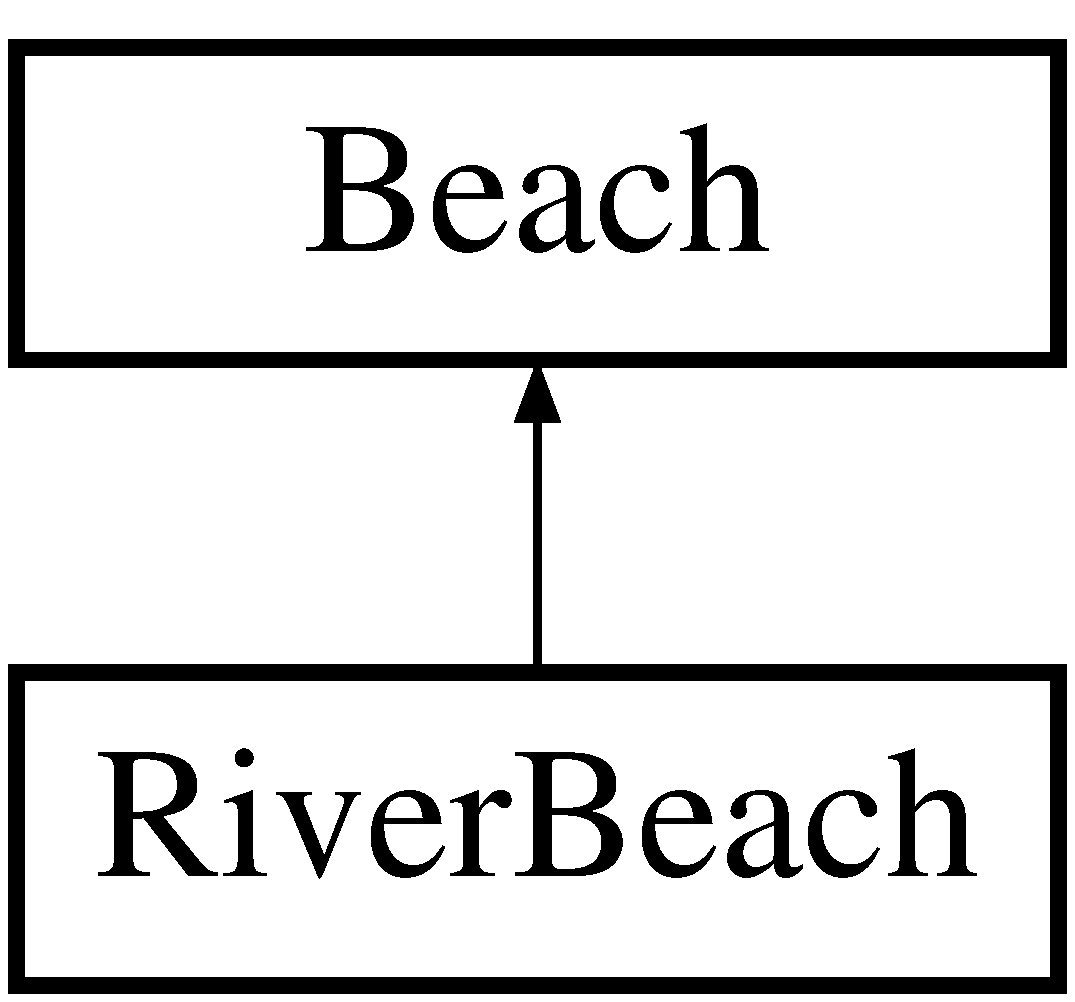
\includegraphics[height=2.000000cm]{class_river_beach}
\end{center}
\end{figure}
\subsection*{Public Member Functions}
\begin{DoxyCompactItemize}
\item 
\hyperlink{class_river_beach_aa4964f12fe275b47b78fa5f1c52b0b32}{River\+Beach} (string \&county, string \&name, bool \&blueflag, bool \&lifeguard, unsigned long \&max\+\_\+capacity, float \&lat, float \&longi, float \&width, float \&max\+Depth)
\begin{DoxyCompactList}\small\item\em Constructor for class \hyperlink{class_river_beach}{River\+Beach}. \end{DoxyCompactList}\item 
\hyperlink{class_river_beach_a70e712f116a7cb499cd9f274dffaa308}{River\+Beach} (string beach)
\begin{DoxyCompactList}\small\item\em Helper construtor which recognizes and associates \hyperlink{class_beach}{Beach}\textquotesingle{}s object\textquotesingle{}s given attributes. \end{DoxyCompactList}\item 
string \hyperlink{class_river_beach_a07f48c077de96aca001f47ce06253f2f}{get\+Type} () const
\begin{DoxyCompactList}\small\item\em Helps identifying from which derived class ths object is. \end{DoxyCompactList}\item 
float \hyperlink{class_river_beach_a4fc528a34d80e3e2a6a48e53ab3e3f49}{get\+\_\+width} () const
\item 
float \hyperlink{class_river_beach_a0bb0a4f13ad1e2d7576d5ef641057e11}{get\+\_\+max\+Depth} () const
\item 
float \hyperlink{class_river_beach_a4bd144e5631968ed671051a203f1bce3}{get\+\_\+aquatic\+Area} () const
\item 
void \hyperlink{class_river_beach_a53697d96e65d8841e5979d3f5d79c9e3}{set\+\_\+width} (float width)
\begin{DoxyCompactList}\small\item\em Changes width. \end{DoxyCompactList}\item 
void \hyperlink{class_river_beach_a1118c334abeeae8352ecaf0f33059f6a}{set\+\_\+max\+Depth} (float max\+Dept)
\begin{DoxyCompactList}\small\item\em Changes maximum depth. \end{DoxyCompactList}\item 
void \hyperlink{class_river_beach_ac236cb64cc422eea722bb99fdb29d4d0}{set\+\_\+aquatic\+Area} (float aquatic\+Area)
\begin{DoxyCompactList}\small\item\em Changes aquatic area. \end{DoxyCompactList}\item 
\mbox{\Hypertarget{class_river_beach_a1dba28cdd6d3c2dda666eb9f398cabbf}\label{class_river_beach_a1dba28cdd6d3c2dda666eb9f398cabbf}} 
void \hyperlink{class_river_beach_a1dba28cdd6d3c2dda666eb9f398cabbf}{display\+Beach} ()
\begin{DoxyCompactList}\small\item\em Displays all information about the beach. \end{DoxyCompactList}\item 
void \hyperlink{class_river_beach_acdbf29ab6540a2b0a5fd18cbea14375b}{write\+Beach} (ofstream \&file) const
\begin{DoxyCompactList}\small\item\em Writes information about the beach in .txt file. \end{DoxyCompactList}\end{DoxyCompactItemize}
\subsection*{Additional Inherited Members}


\subsection{Constructor \& Destructor Documentation}
\mbox{\Hypertarget{class_river_beach_aa4964f12fe275b47b78fa5f1c52b0b32}\label{class_river_beach_aa4964f12fe275b47b78fa5f1c52b0b32}} 
\index{River\+Beach@{River\+Beach}!River\+Beach@{River\+Beach}}
\index{River\+Beach@{River\+Beach}!River\+Beach@{River\+Beach}}
\subsubsection{\texorpdfstring{River\+Beach()}{RiverBeach()}\hspace{0.1cm}{\footnotesize\ttfamily [1/2]}}
{\footnotesize\ttfamily River\+Beach\+::\+River\+Beach (\begin{DoxyParamCaption}\item[{string \&}]{county,  }\item[{string \&}]{name,  }\item[{bool \&}]{blueflag,  }\item[{bool \&}]{lifeguard,  }\item[{unsigned long \&}]{max\+\_\+capacity,  }\item[{float \&}]{lat,  }\item[{float \&}]{longi,  }\item[{float \&}]{width,  }\item[{float \&}]{max\+Depth }\end{DoxyParamCaption})}



Constructor for class \hyperlink{class_river_beach}{River\+Beach}. 


\begin{DoxyParams}{Parameters}
{\em county} & \\
\hline
{\em name} & \\
\hline
{\em blueflag} & \\
\hline
{\em lifeguard} & \\
\hline
{\em max\+\_\+capacity} & \\
\hline
{\em lat} & \\
\hline
{\em longi} & \\
\hline
{\em width} & \\
\hline
{\em max\+Depth} & \\
\hline
{\em basic\+Services} & \\
\hline
\end{DoxyParams}
\mbox{\Hypertarget{class_river_beach_a70e712f116a7cb499cd9f274dffaa308}\label{class_river_beach_a70e712f116a7cb499cd9f274dffaa308}} 
\index{River\+Beach@{River\+Beach}!River\+Beach@{River\+Beach}}
\index{River\+Beach@{River\+Beach}!River\+Beach@{River\+Beach}}
\subsubsection{\texorpdfstring{River\+Beach()}{RiverBeach()}\hspace{0.1cm}{\footnotesize\ttfamily [2/2]}}
{\footnotesize\ttfamily River\+Beach\+::\+River\+Beach (\begin{DoxyParamCaption}\item[{string}]{beach }\end{DoxyParamCaption})}



Helper construtor which recognizes and associates \hyperlink{class_beach}{Beach}\textquotesingle{}s object\textquotesingle{}s given attributes. 


\begin{DoxyParams}{Parameters}
{\em line} & from txt file representing an object of class beach \\
\hline
\end{DoxyParams}


\subsection{Member Function Documentation}
\mbox{\Hypertarget{class_river_beach_a4bd144e5631968ed671051a203f1bce3}\label{class_river_beach_a4bd144e5631968ed671051a203f1bce3}} 
\index{River\+Beach@{River\+Beach}!get\+\_\+aquatic\+Area@{get\+\_\+aquatic\+Area}}
\index{get\+\_\+aquatic\+Area@{get\+\_\+aquatic\+Area}!River\+Beach@{River\+Beach}}
\subsubsection{\texorpdfstring{get\+\_\+aquatic\+Area()}{get\_aquaticArea()}}
{\footnotesize\ttfamily float River\+Beach\+::get\+\_\+aquatic\+Area (\begin{DoxyParamCaption}{ }\end{DoxyParamCaption}) const\hspace{0.3cm}{\ttfamily [inline]}, {\ttfamily [virtual]}}

\begin{DoxyReturn}{Returns}
aquatic area 
\end{DoxyReturn}


Implements \hyperlink{class_beach_afc6a57f98777ec5de1882acaf2703e6d}{Beach}.

\mbox{\Hypertarget{class_river_beach_a0bb0a4f13ad1e2d7576d5ef641057e11}\label{class_river_beach_a0bb0a4f13ad1e2d7576d5ef641057e11}} 
\index{River\+Beach@{River\+Beach}!get\+\_\+max\+Depth@{get\+\_\+max\+Depth}}
\index{get\+\_\+max\+Depth@{get\+\_\+max\+Depth}!River\+Beach@{River\+Beach}}
\subsubsection{\texorpdfstring{get\+\_\+max\+Depth()}{get\_maxDepth()}}
{\footnotesize\ttfamily float River\+Beach\+::get\+\_\+max\+Depth (\begin{DoxyParamCaption}{ }\end{DoxyParamCaption}) const\hspace{0.3cm}{\ttfamily [inline]}, {\ttfamily [virtual]}}

\begin{DoxyReturn}{Returns}
maximun depth 
\end{DoxyReturn}


Implements \hyperlink{class_beach_a5942f7aa56af3b61d2974a754913ab7e}{Beach}.

\mbox{\Hypertarget{class_river_beach_a4fc528a34d80e3e2a6a48e53ab3e3f49}\label{class_river_beach_a4fc528a34d80e3e2a6a48e53ab3e3f49}} 
\index{River\+Beach@{River\+Beach}!get\+\_\+width@{get\+\_\+width}}
\index{get\+\_\+width@{get\+\_\+width}!River\+Beach@{River\+Beach}}
\subsubsection{\texorpdfstring{get\+\_\+width()}{get\_width()}}
{\footnotesize\ttfamily float River\+Beach\+::get\+\_\+width (\begin{DoxyParamCaption}{ }\end{DoxyParamCaption}) const\hspace{0.3cm}{\ttfamily [inline]}, {\ttfamily [virtual]}}

\begin{DoxyReturn}{Returns}
width; 
\end{DoxyReturn}


Implements \hyperlink{class_beach_af28e3603ea98766d94c9e8eb9f76d509}{Beach}.

\mbox{\Hypertarget{class_river_beach_a07f48c077de96aca001f47ce06253f2f}\label{class_river_beach_a07f48c077de96aca001f47ce06253f2f}} 
\index{River\+Beach@{River\+Beach}!get\+Type@{get\+Type}}
\index{get\+Type@{get\+Type}!River\+Beach@{River\+Beach}}
\subsubsection{\texorpdfstring{get\+Type()}{getType()}}
{\footnotesize\ttfamily string River\+Beach\+::get\+Type (\begin{DoxyParamCaption}{ }\end{DoxyParamCaption}) const\hspace{0.3cm}{\ttfamily [inline]}, {\ttfamily [virtual]}}



Helps identifying from which derived class ths object is. 

\begin{DoxyReturn}{Returns}
\char`\"{}\+Bayou\+Beach\char`\"{} if it\textquotesingle{}s a class \hyperlink{class_bayou_beach}{Bayou\+Beach} object, \char`\"{}\+River\+Beach\char`\"{} if it\textquotesingle{}s a class \hyperlink{class_river_beach}{River\+Beach} object 
\end{DoxyReturn}


Implements \hyperlink{class_beach_a30001df535b2456e47611c7a0705660b}{Beach}.

\mbox{\Hypertarget{class_river_beach_ac236cb64cc422eea722bb99fdb29d4d0}\label{class_river_beach_ac236cb64cc422eea722bb99fdb29d4d0}} 
\index{River\+Beach@{River\+Beach}!set\+\_\+aquatic\+Area@{set\+\_\+aquatic\+Area}}
\index{set\+\_\+aquatic\+Area@{set\+\_\+aquatic\+Area}!River\+Beach@{River\+Beach}}
\subsubsection{\texorpdfstring{set\+\_\+aquatic\+Area()}{set\_aquaticArea()}}
{\footnotesize\ttfamily void River\+Beach\+::set\+\_\+aquatic\+Area (\begin{DoxyParamCaption}\item[{float}]{aquatic\+Area }\end{DoxyParamCaption})\hspace{0.3cm}{\ttfamily [inline]}, {\ttfamily [virtual]}}



Changes aquatic area. 


\begin{DoxyParams}{Parameters}
{\em Aquatic} & area \\
\hline
\end{DoxyParams}


Implements \hyperlink{class_beach_a37e71c3348356d49f3b1080973708376}{Beach}.

\mbox{\Hypertarget{class_river_beach_a1118c334abeeae8352ecaf0f33059f6a}\label{class_river_beach_a1118c334abeeae8352ecaf0f33059f6a}} 
\index{River\+Beach@{River\+Beach}!set\+\_\+max\+Depth@{set\+\_\+max\+Depth}}
\index{set\+\_\+max\+Depth@{set\+\_\+max\+Depth}!River\+Beach@{River\+Beach}}
\subsubsection{\texorpdfstring{set\+\_\+max\+Depth()}{set\_maxDepth()}}
{\footnotesize\ttfamily void River\+Beach\+::set\+\_\+max\+Depth (\begin{DoxyParamCaption}\item[{float}]{max\+Dept }\end{DoxyParamCaption})\hspace{0.3cm}{\ttfamily [inline]}, {\ttfamily [virtual]}}



Changes maximum depth. 


\begin{DoxyParams}{Parameters}
{\em maximum} & depth \\
\hline
\end{DoxyParams}


Implements \hyperlink{class_beach_af0226438bc6e731b2bca9f5a6078b572}{Beach}.

\mbox{\Hypertarget{class_river_beach_a53697d96e65d8841e5979d3f5d79c9e3}\label{class_river_beach_a53697d96e65d8841e5979d3f5d79c9e3}} 
\index{River\+Beach@{River\+Beach}!set\+\_\+width@{set\+\_\+width}}
\index{set\+\_\+width@{set\+\_\+width}!River\+Beach@{River\+Beach}}
\subsubsection{\texorpdfstring{set\+\_\+width()}{set\_width()}}
{\footnotesize\ttfamily void River\+Beach\+::set\+\_\+width (\begin{DoxyParamCaption}\item[{float}]{width }\end{DoxyParamCaption})\hspace{0.3cm}{\ttfamily [inline]}, {\ttfamily [virtual]}}



Changes width. 


\begin{DoxyParams}{Parameters}
{\em width} & \\
\hline
\end{DoxyParams}


Implements \hyperlink{class_beach_a3f3a4bde9008bcc87861710e8c99c008}{Beach}.

\mbox{\Hypertarget{class_river_beach_acdbf29ab6540a2b0a5fd18cbea14375b}\label{class_river_beach_acdbf29ab6540a2b0a5fd18cbea14375b}} 
\index{River\+Beach@{River\+Beach}!write\+Beach@{write\+Beach}}
\index{write\+Beach@{write\+Beach}!River\+Beach@{River\+Beach}}
\subsubsection{\texorpdfstring{write\+Beach()}{writeBeach()}}
{\footnotesize\ttfamily void River\+Beach\+::write\+Beach (\begin{DoxyParamCaption}\item[{ofstream \&}]{file }\end{DoxyParamCaption}) const\hspace{0.3cm}{\ttfamily [virtual]}}



Writes information about the beach in .txt file. 


\begin{DoxyParams}{Parameters}
{\em file} & \\
\hline
\end{DoxyParams}


Implements \hyperlink{class_beach_a2ba3bf80382fa1b5e00befe0c4ccde88}{Beach}.



The documentation for this class was generated from the following files\+:\begin{DoxyCompactItemize}
\item 
/\+Users/beamendes/\+Documents/\+A\+E\+D\+A/\+A\+E\+D\+A-\/\+F\+E\+U\+P/aeda/Beach.\+h\item 
/\+Users/beamendes/\+Documents/\+A\+E\+D\+A/\+A\+E\+D\+A-\/\+F\+E\+U\+P/aeda/Beach.\+cpp\end{DoxyCompactItemize}

\hypertarget{class_services}{}\section{Services Class Reference}
\label{class_services}\index{Services@{Services}}
\subsection*{Public Member Functions}
\begin{DoxyCompactItemize}
\item 
\hyperlink{class_services_ae5a9f9602657bb68fdd380fed0f7a237}{Services} (string type, string name, string price\+Range, string stars)
\begin{DoxyCompactList}\small\item\em Constructor class \hyperlink{class_services}{Services}. \end{DoxyCompactList}\item 
\hyperlink{class_services_a57ccd705c80a34f7c7cd3c35057c6256}{Services} (string service)
\begin{DoxyCompactList}\small\item\em Helper construtor for class \hyperlink{class_services}{Services} which creates an object from information in file. \end{DoxyCompactList}\item 
\mbox{\Hypertarget{class_services_ac158976e8d9bd44be7e5959452b13178}\label{class_services_ac158976e8d9bd44be7e5959452b13178}} 
\hyperlink{class_services_ac158976e8d9bd44be7e5959452b13178}{Services} ()
\begin{DoxyCompactList}\small\item\em Alternative constructor. \end{DoxyCompactList}\item 
string \hyperlink{class_services_af4da1cfed2bfabfc164d505993d105ce}{get\+Type} ()
\item 
string \hyperlink{class_services_a71c420517519b0316b771c637044b76a}{get\+Name} ()
\item 
string \hyperlink{class_services_ac4c520cb327c737a775be426ffae1165}{get\+Price\+Range} ()
\item 
string \hyperlink{class_services_a35360c22f682d48fd7271f9c5017c7a5}{get\+Stars} ()
\item 
void \hyperlink{class_services_ad299f8ec3b29a5fffc513ae9b89e4c1d}{set\+Type} (string type)
\item 
void \hyperlink{class_services_a68e4ebe3d329da8ffd56cea463fb1c80}{set\+Name} (string name)
\item 
void \hyperlink{class_services_a883f71c238f82e77c01f244ded84dd57}{set\+Price\+Range} (string price)
\item 
void \hyperlink{class_services_a4cc0854b2f6bbb357f4e14d4ed753d2d}{set\+Stars} (string stars)
\end{DoxyCompactItemize}


\subsection{Constructor \& Destructor Documentation}
\mbox{\Hypertarget{class_services_ae5a9f9602657bb68fdd380fed0f7a237}\label{class_services_ae5a9f9602657bb68fdd380fed0f7a237}} 
\index{Services@{Services}!Services@{Services}}
\index{Services@{Services}!Services@{Services}}
\subsubsection{\texorpdfstring{Services()}{Services()}\hspace{0.1cm}{\footnotesize\ttfamily [1/2]}}
{\footnotesize\ttfamily Services\+::\+Services (\begin{DoxyParamCaption}\item[{string}]{type,  }\item[{string}]{name,  }\item[{string}]{price\+Range,  }\item[{string}]{stars }\end{DoxyParamCaption})}



Constructor class \hyperlink{class_services}{Services}. 


\begin{DoxyParams}{Parameters}
{\em type} & \\
\hline
{\em name} & \\
\hline
{\em price\+Range} & \\
\hline
{\em stars} & \\
\hline
\end{DoxyParams}
\mbox{\Hypertarget{class_services_a57ccd705c80a34f7c7cd3c35057c6256}\label{class_services_a57ccd705c80a34f7c7cd3c35057c6256}} 
\index{Services@{Services}!Services@{Services}}
\index{Services@{Services}!Services@{Services}}
\subsubsection{\texorpdfstring{Services()}{Services()}\hspace{0.1cm}{\footnotesize\ttfamily [2/2]}}
{\footnotesize\ttfamily Services\+::\+Services (\begin{DoxyParamCaption}\item[{string}]{service }\end{DoxyParamCaption})}



Helper construtor for class \hyperlink{class_services}{Services} which creates an object from information in file. 


\begin{DoxyParams}{Parameters}
{\em string} & containing service attributes separated by collumns \\
\hline
\end{DoxyParams}


\subsection{Member Function Documentation}
\mbox{\Hypertarget{class_services_a71c420517519b0316b771c637044b76a}\label{class_services_a71c420517519b0316b771c637044b76a}} 
\index{Services@{Services}!get\+Name@{get\+Name}}
\index{get\+Name@{get\+Name}!Services@{Services}}
\subsubsection{\texorpdfstring{get\+Name()}{getName()}}
{\footnotesize\ttfamily string Services\+::get\+Name (\begin{DoxyParamCaption}{ }\end{DoxyParamCaption})\hspace{0.3cm}{\ttfamily [inline]}}

\begin{DoxyReturn}{Returns}
name 
\end{DoxyReturn}
\mbox{\Hypertarget{class_services_ac4c520cb327c737a775be426ffae1165}\label{class_services_ac4c520cb327c737a775be426ffae1165}} 
\index{Services@{Services}!get\+Price\+Range@{get\+Price\+Range}}
\index{get\+Price\+Range@{get\+Price\+Range}!Services@{Services}}
\subsubsection{\texorpdfstring{get\+Price\+Range()}{getPriceRange()}}
{\footnotesize\ttfamily string Services\+::get\+Price\+Range (\begin{DoxyParamCaption}{ }\end{DoxyParamCaption})\hspace{0.3cm}{\ttfamily [inline]}}

\begin{DoxyReturn}{Returns}
price range 
\end{DoxyReturn}
\mbox{\Hypertarget{class_services_a35360c22f682d48fd7271f9c5017c7a5}\label{class_services_a35360c22f682d48fd7271f9c5017c7a5}} 
\index{Services@{Services}!get\+Stars@{get\+Stars}}
\index{get\+Stars@{get\+Stars}!Services@{Services}}
\subsubsection{\texorpdfstring{get\+Stars()}{getStars()}}
{\footnotesize\ttfamily string Services\+::get\+Stars (\begin{DoxyParamCaption}{ }\end{DoxyParamCaption})\hspace{0.3cm}{\ttfamily [inline]}}

\begin{DoxyReturn}{Returns}
stars 
\end{DoxyReturn}
\mbox{\Hypertarget{class_services_af4da1cfed2bfabfc164d505993d105ce}\label{class_services_af4da1cfed2bfabfc164d505993d105ce}} 
\index{Services@{Services}!get\+Type@{get\+Type}}
\index{get\+Type@{get\+Type}!Services@{Services}}
\subsubsection{\texorpdfstring{get\+Type()}{getType()}}
{\footnotesize\ttfamily string Services\+::get\+Type (\begin{DoxyParamCaption}{ }\end{DoxyParamCaption})\hspace{0.3cm}{\ttfamily [inline]}}

\begin{DoxyReturn}{Returns}
type 
\end{DoxyReturn}
\mbox{\Hypertarget{class_services_a68e4ebe3d329da8ffd56cea463fb1c80}\label{class_services_a68e4ebe3d329da8ffd56cea463fb1c80}} 
\index{Services@{Services}!set\+Name@{set\+Name}}
\index{set\+Name@{set\+Name}!Services@{Services}}
\subsubsection{\texorpdfstring{set\+Name()}{setName()}}
{\footnotesize\ttfamily void Services\+::set\+Name (\begin{DoxyParamCaption}\item[{string}]{name }\end{DoxyParamCaption})\hspace{0.3cm}{\ttfamily [inline]}}

Changes name. 
\begin{DoxyParams}{Parameters}
{\em name} & \\
\hline
\end{DoxyParams}
\mbox{\Hypertarget{class_services_a883f71c238f82e77c01f244ded84dd57}\label{class_services_a883f71c238f82e77c01f244ded84dd57}} 
\index{Services@{Services}!set\+Price\+Range@{set\+Price\+Range}}
\index{set\+Price\+Range@{set\+Price\+Range}!Services@{Services}}
\subsubsection{\texorpdfstring{set\+Price\+Range()}{setPriceRange()}}
{\footnotesize\ttfamily void Services\+::set\+Price\+Range (\begin{DoxyParamCaption}\item[{string}]{price }\end{DoxyParamCaption})\hspace{0.3cm}{\ttfamily [inline]}}

Changes price range. 
\begin{DoxyParams}{Parameters}
{\em price} & \\
\hline
\end{DoxyParams}
\mbox{\Hypertarget{class_services_a4cc0854b2f6bbb357f4e14d4ed753d2d}\label{class_services_a4cc0854b2f6bbb357f4e14d4ed753d2d}} 
\index{Services@{Services}!set\+Stars@{set\+Stars}}
\index{set\+Stars@{set\+Stars}!Services@{Services}}
\subsubsection{\texorpdfstring{set\+Stars()}{setStars()}}
{\footnotesize\ttfamily void Services\+::set\+Stars (\begin{DoxyParamCaption}\item[{string}]{stars }\end{DoxyParamCaption})\hspace{0.3cm}{\ttfamily [inline]}}

Changes stars. 
\begin{DoxyParams}{Parameters}
{\em stars} & \\
\hline
\end{DoxyParams}
\mbox{\Hypertarget{class_services_ad299f8ec3b29a5fffc513ae9b89e4c1d}\label{class_services_ad299f8ec3b29a5fffc513ae9b89e4c1d}} 
\index{Services@{Services}!set\+Type@{set\+Type}}
\index{set\+Type@{set\+Type}!Services@{Services}}
\subsubsection{\texorpdfstring{set\+Type()}{setType()}}
{\footnotesize\ttfamily void Services\+::set\+Type (\begin{DoxyParamCaption}\item[{string}]{type }\end{DoxyParamCaption})\hspace{0.3cm}{\ttfamily [inline]}}

Changes type. 
\begin{DoxyParams}{Parameters}
{\em type} & \\
\hline
\end{DoxyParams}


The documentation for this class was generated from the following files\+:\begin{DoxyCompactItemize}
\item 
/\+Users/beamendes/\+Documents/\+A\+E\+D\+A/\+A\+E\+D\+A-\/\+F\+E\+U\+P/aeda/Services.\+h\item 
/\+Users/beamendes/\+Documents/\+A\+E\+D\+A/\+A\+E\+D\+A-\/\+F\+E\+U\+P/aeda/Services.\+cpp\end{DoxyCompactItemize}

%--- End generated contents ---

% Index
\backmatter
\newpage
\phantomsection
\clearemptydoublepage
\addcontentsline{toc}{chapter}{Index}
\printindex

\end{document}
